\tikzset{every picture/.style={line width=0.75pt}} %set default line width to 0.75pt        

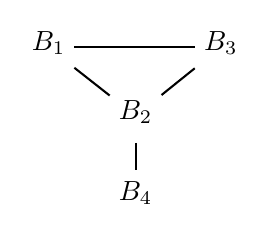
\begin{tikzpicture}[x=0.75pt,y=0.75pt,yscale=-1,xscale=1]
%uncomment if require: \path (0,534); %set diagram left start at 0, and has height of 534


% Text Node
\draw (20,22) node [anchor=north west][inner sep=0.75pt]    {$B_{1}$};
% Text Node
\draw (62,55) node [anchor=north west][inner sep=0.75pt]    {$B_{2}$};
% Text Node
\draw (103,22) node [anchor=north west][inner sep=0.75pt]    {$B_{3}$};
% Text Node
\draw (62,94) node [anchor=north west][inner sep=0.75pt]    {$B_{4}$};
% Connection
\draw    (100,31) -- (42,31) ;
% Connection
\draw    (59,54.18) -- (42,40.82) ;
% Connection
\draw    (84,53.94) -- (100,41.06) ;
% Connection
\draw    (71.5,77) -- (71.5,90) ;

\end{tikzpicture}